\documentclass[12pt]{article}
\usepackage{graphicx}
\usepackage[margin=1in]{geometry}

\title{Fast All-Pair Shortest Path Algorithms on \\ Big Unweighted, Undirected Graph}
\author{Junming Wang, Boo Kai Hsien}

\begin{document}
\maketitle
\pagebreak

\section{Algorithms}

We have considered 4 main algorithms:

\begin{itemize}
	\item BFS
	\item Cache-efficient BFS
	\item Cache-efficient BFS Modified
	\item Seidel's algorithm
\end{itemize}

The first 3 algorithms are for single-source shortest path problem, so we ran it from each node to solve the problem. 

\subsection{Cache-efficient BFS Modified}

Since we need to run $n$ instances of the cache-efficient BFS, we try to see if there is any pre-processing we can make to improve the current algorithm. We focus on the part where we merge all neighbors of nodes in $L_i$.

First of all, we sort the neighbors in the adjacency list for each node. Then, when we are merging $k$ lists of neighbors, the problem is the same as to merge $k$ number of sorted list. Merging two lists of size $n$ takes $O(n)$ time. If we recursively merge the first half and the second half of the lists. We get a running time of

$$T(n,k) = T(2n, k/2) + nk = O(nk\log(k))$$

Our merge is cache-efficient, and the number of cache-references is

$$T(n,k) = T(2n, k/2) + nk / B = O(nk \log(k)/ B)$$

\subsection{Seidel's Algorithm}

Seidel's algorithm is an all-pair shortest path algorithm for unweighted and undirected graphs. It has a running time of $O(\texttt{MATMUL}(n)\log n)$ where $\texttt{MATMUL}(n)$ is the time needed to multiply two matrices of size $n\times n$.

We are unable to run Seidel's algorithm on graph size more than $3000$ nodes because of its recursive nature and consumes too much memory. However, we are able to run it on smaller graphs to compare with the other algorithms.

\pagebreak

\section{Results}

\subsection{Running Time}

Here is the result of comparing the three algorithms: BFS, Cache-efficient BFS and Cache-efficient BFS Modified. The algorithm is tested on graphs with $10000$ nodes and $10000$, $100000$, $1000000$ and $10000000$ edges respectively. The y-axis is the log-scaled running time. For example, the value $10$ indicates a running time of $2^{10} = 1024$ seconds.

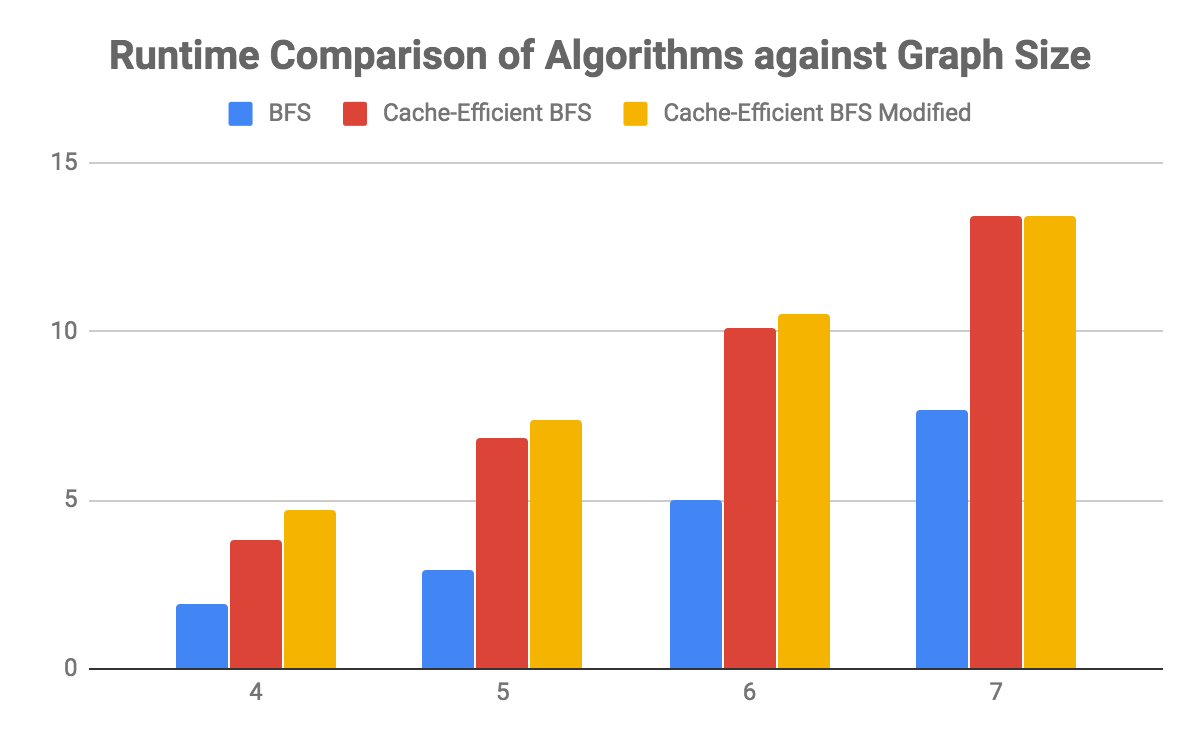
\includegraphics[scale=0.4]{graph-1}

The performance of Cache-efficient BFS agrees with what we learned in the lecture. It works much more better for sparse graph. As the number of edges increase, the ratio between the running time of cache-efficient BFS and usual BFS increases.

One interesting result is that our modified cache-efficient BFS starts to perform better than the cache-efficient BFS on dense graph (it is better when number of edges is $10^7$).

\pagebreak

\subsection{Cache Miss Rate}

Even though our cache-efficient BFS is worse than the normal BFS, we can see improvements on the cache miss rate. Here is a similar graph except we measure the cache miss rates.

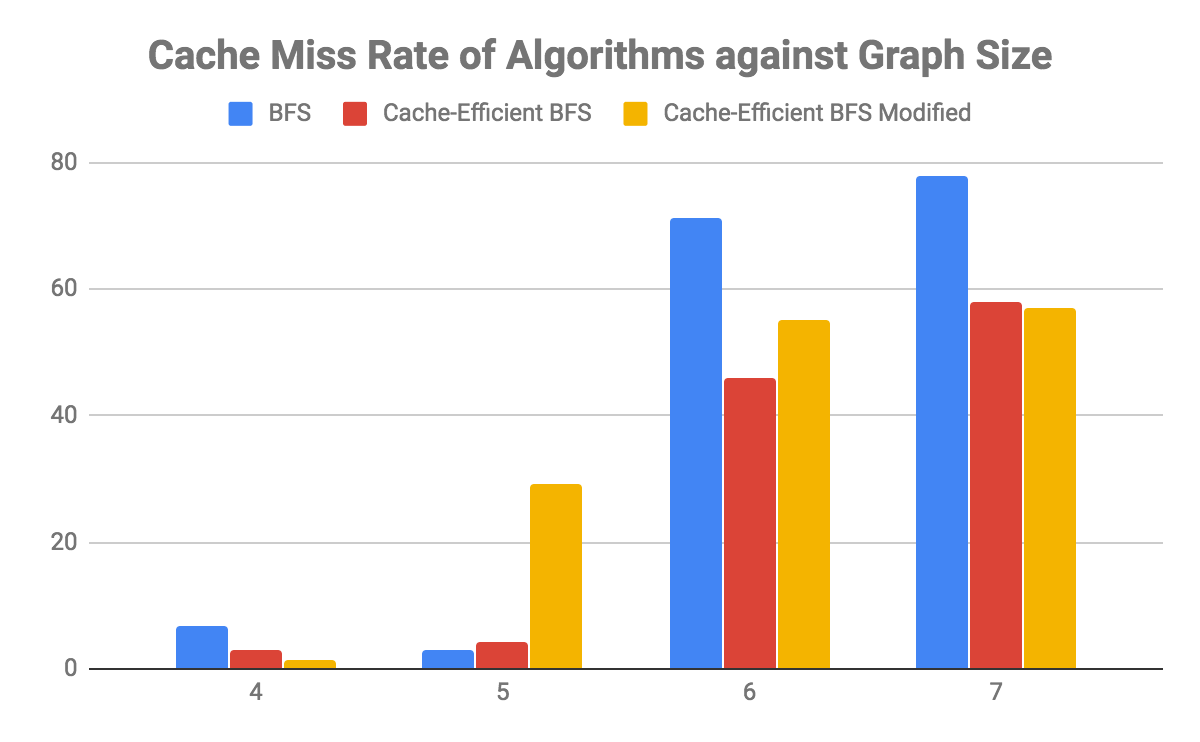
\includegraphics[scale=0.4]{graph-2}

As can be seen from the graph, the number of cache misses for both cache-efficient BFSs outperform the normal BFS when the graph size is larger.

We notice an inconsistent behavior when the number of edges is $10^5$. The cache-efficient BFS has higher cache-miss rate and our modified cache-efficient has even higher cache-miss rate. Unfortunately, we were unable to find out the reason before the submission of this report.

Similar to the running time performance, our modified BFS performs better than the cache-efficient BFS when the graph is dense.

\subsection{Real World Dataset}

The source of our real world dataset is from Stanford Large Network Dataset Collection. We used anonymised social circles from Facebook because it fits our graph criteria: unweighted and undirected. It has 4039 nodes and 88234 edges.

\pagebreak

\section{Discussions}

Here we discuss things that we have done and found interesting throughout the course of this project. You may focus only on the relevant sections :)

\subsection{Analysis of Cache-Efficient BFS Modified}

Using the cache model from lecture we can see that merging two sorted list of length $n_1$ and $n_2$ has cost $O((n_1+n_2)/B)$.

Assume we are merging $k$ sorted lists of length $n$. We recursively merge two lists until we have only 1 list left (as described in section 1.1). Merging $|L_i|$ lists of average length $E(L_i) / |L_i|$ into $|L_i|/2$ lists of average length $2E(L_i)/|L_i|$ costs $O(E(L_i)/B)$, thus the total cost of merging $L_i$ sorted list of length $E(L_i)/|L_i|$ is $O(E(L_i)\log(|L_i|) / B$ as a result of:

$$T(|L_i|, E(L_i)/|L_i|) = T(|L_i|/2, 2E(L_i)/|L_i|) + O(E(L_i)/B)$$

This performance of this part is compared with the cache-efficient BFS we learned in class, which has cost $O(\texttt{SORT}(E(L_i))=O((E(L_i)/B)\log_{M/B}(E(L_i)/B))$.

Thus the trade off is between $\log(|L_i|)$ and $\log_{M/B}{(E(L_i)/B)}$. This explains why our version is better in dense graph, when $E(L_i)$ is huge. In this case, the pre-processing time is $n\texttt{SORT}(n)\approx \texttt{SORT}(|E|)$.

\subsection{Random Graph Generator}

We are interested in seeing how the running time or cache miss rate differs for different graph parameters, so we need to generate our own graphs. Here is a short description on the algorithm.

We first generate a spanning tree, and then randomly add edges until we hit the number we desired. The algorithm for generating a spanning tree is very simple. To create a spanning tree of $n$ nodes labeled $0$ to $n-1$, we first create a vector of size storing all the node labels. Then, we randomly shuffle the vector (using STL or the Fisher-Yates learned in CS2020). Next, for node $1$ to $n-1$, we add an edge from it to one of the node on its left in the vector. Since there is only $n-1$ edges, and there is no cycle, it must be a spanning tree.

\subsection{Cache Miss Rate Measurement}

We use following command to measure the number of cache-refereces, cache-misses and instructions for a process.

\begin{verbatim}
perf stat -e cache-references -e cache-misses -e instructions <executable>
\end{verbatim}

\pagebreak

\section{Conclusion}

We have arrived at several conclusions for this project. Even though the results suggest that the normal BFS runs faster, in the case where cache-miss is very expensive, the cache-efficient BFSs is preferred. Furthermore, if the graph is dense, our version of BFS should be used instead.

\end{document}
